\testfile{pgfplotstest.expr.tex}
\testsection{`plot expression' test}
\testsubsection{sin(x)}
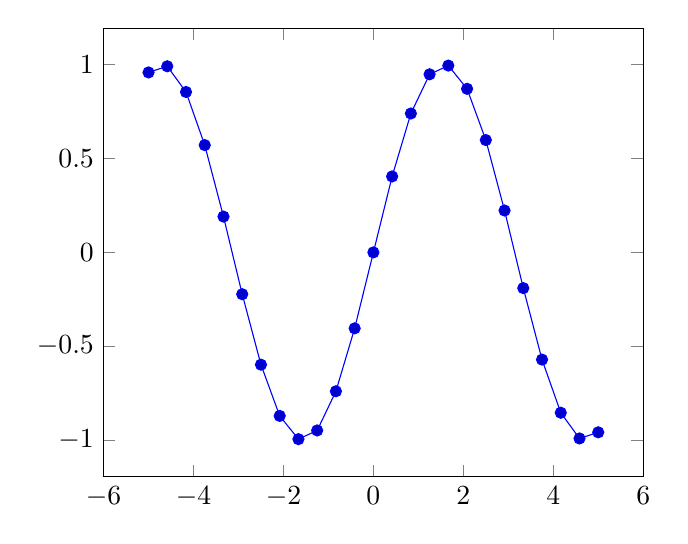
\begin{tikzpicture}
\begin{axis}
\addplot (\x,{sin(\x r)});
\end{axis}
\end{tikzpicture}

\testsubsection{$x^2$}
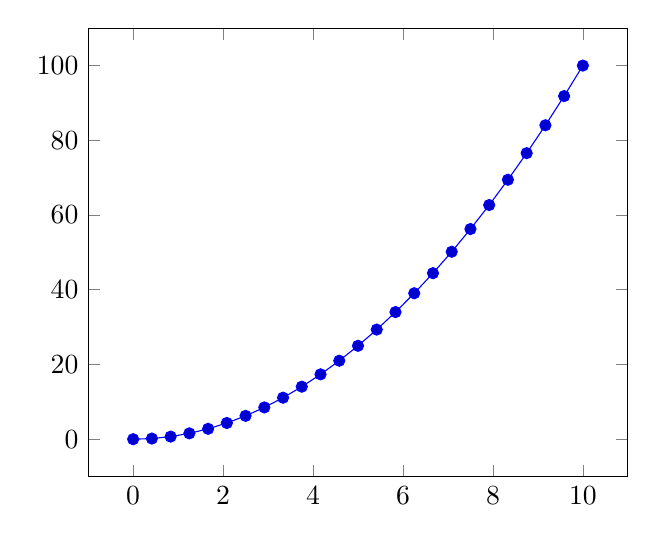
\begin{tikzpicture}
\begin{axis}
\addplot plot[domain=0:10] (\x,\x^2);
\end{axis}
\end{tikzpicture}

\def\testexpression#1#2{%
	\testsubsection{$#1$}
	\begin{tikzpicture}
		\begin{axis}[title={$#1$},#2]
			\addplot {#1};
		\end{axis}
	\end{tikzpicture}%
}%
\def\testgnuplot#1#2{%
	\begin{tikzpicture}
		\begin{axis}[title={$#1$},#2]
			\addplot gnuplot {#1};
		\end{axis}
	\end{tikzpicture}%
}%


\testexpression{x^10}{domain=-3:3}

\testexpression{x^10}{domain=-3:3000}

\testexpression{x*5*(1-100)/(1-x)}{domain=1000:3000}

Das liegt an der relativen genauigkeit und an der enge des datenbereichs:

gnuplopt:

\testgnuplot{x*5*(1-100)/(1-x)}{domain=1000:3000}

\testexpression{x*5*(1-100)/(1-x)}{domain=20:3000}

\testexpression{1/x}{domain=1e-10:1e-9,samples=300}

\testexpression{exp(0-(x-90)^2/0.0001)}{domain=89.9:90.1,samples=300}

\testexpression{sqrt(abs(x))}{domain=-3:3,samples=501}

